\documentclass[answers,dvipsnames]{exam}
\usepackage{marvosym}

%...TikZ & PGF
\usepackage{pgfplots}
\pgfplotsset{compat=1.11}
\tikzset{>=latex}
\usetikzlibrary{calc,math}
\usepackage{tikzsymbols}
\usepgfplotslibrary{fillbetween}
\usetikzlibrary{decorations.markings} 
\usetikzlibrary{arrows.meta} %...APP2 for arrows as objects and images
\usetikzlibrary{backgrounds} %...For shading portions of graphs
\usetikzlibrary{patterns} %...Unit 5 Problems
\usetikzlibrary{shapes.geometric} %...For drawing cylinders in Unit 2
\tikzset{
    mark position/.style args={#1(#2)}{
        postaction={
            decorate,
            decoration={
                markings,
                mark=at position #1 with \coordinate (#2);
            }
        }
    }
} %...See https://tex.stackexchange.com/questions/43960/define-node-at-relative-coordinates-of-draw-plot

\tikzset{
    declare function = {trajectoryequation10(\x,\vi,\thetai)= tan(\thetai)*\x - 10*\x^2/(2*(\vi*cos(\thetai))^2);},
    declare function = {trajectoryequation(\x,\vi,\thetai)= tan(\thetai)*\x - 9.8*\x^2/(2*(\vi*cos(\thetai))^2);},
    declare function = {patheq(\x,\yi,\vi,\thetai)= \yi + tan(\thetai)*\x - 9.8*\x^2/(2*(\vi*cos(\thetai))^2);},
    declare function = {patheqten(\x,\yi,\vi,\thetai)= \yi + tan(\thetai)*\x - 10*\x^2/(2*(\vi*cos(\thetai))^2);} %like patheq but with gravity = 10
}

%...siunitx
\usepackage{siunitx}
\DeclareSIUnit{\nothing}{\relax}
\def\mymu{\SI{}{\micro\nothing} }
\DeclareSIUnit\mmHg{mmHg}
\DeclareSIUnit{\mile}{mi}
%...NOTE: "The product symbol between the number and unit is set using the quantity-product option."

%...Other
\usepackage{amsthm}
\usepackage{amsmath}
\usepackage{amssymb}
\usepackage{cancel}
\usepackage{subcaption}
\usepackage{dashrule}
\usepackage{enumitem}
\usepackage{fontawesome}
\usepackage{multicol}
\usepackage{glossaries}
%\numberwithin{equation}{section}
\numberwithin{figure}{section}
\usepackage{float}
\usepackage{twemojis} %...twitter emojis
\usepackage{utfsym}
\newcommand{\R}{\mathbb{R}} %...real number symbol
\usepackage{graphicx}
\graphicspath{ {../Figures/} }
\usepackage{hyperref}
\hypersetup{colorlinks=true,
    linkcolor=blue,
    filecolor=magenta,
    urlcolor=cyan,}
\urlstyle{same}
\newcommand{\hdashline}{{\hdashrule{\textwidth}{0.5pt}{0.8mm}}}
\newcommand{\hgraydashline}{{\color{lightgray} \hdashrule{0.99\textwidth}{1pt}{0.8mm}}}

%...Miscellaneous user-defined symbols
\newcommand{\fnet}{F_{\text{net}}} %...For net force
\newcommand{\bvec}[1]{\vec{\mathbf{#1}}} %...bold vector
\newcommand{\bhat}[1]{\,\hat{\mathbf{#1}}} %...bold hat vector
\newcommand{\que}{\mathord{?}}  %...Question mark symbol in equation env
%...Define thick horizontal rule for examples:
\newcommand{\hhrule}{\hrule\hrule}
\let\oldtexttt\texttt% Store \texttt
\renewcommand{\texttt}[2][black]{\textcolor{#1}{\ttfamily #2}}% 

%...For use in the exam document class
\newif\ifprintmetasolutions


%...Decreases space above and below align and gather enironment
\makeatletter
\g@addto@macro\normalsize{%
  \setlength\abovedisplayskip{-3pt}
  \setlength\belowdisplayskip{6pt} 
}
\makeatother





\usepackage[margin=1in]{geometry}
\usepackage[figurewithin=none]{caption}
\usepackage{exam-randomizechoices}

\CorrectChoiceEmphasis{\color{red}\bfseries}
\renewcommand{\solutiontitle}{\noindent\textbf{\textcolor{red}{Solution:}}\enspace}

\usepackage{OutilsGeomTikz}
\usepackage{utfsym} %...Symbols in Unit 7 Problems
\usepackage{tabu} %...Symbols in Unit 7 Problems

%...For use in Unit 2            %    
\setlength{\columnsep}{2cm}      %
\setlength{\columnseprule}{1pt}  %
\usepackage[none]{hyphenat}      %
%%%%%%%%%%%%%%%%%%%%%%%%%%%%%%%%%

%...For use in Unit 11 on Waves:
\pgfdeclarehorizontalshading{visiblelight}{50bp}{  %
color(0.00000000000000bp)=(red);                   %
color(8.33333333333333bp)=(orange);                %
color(16.66666666666670bp)=(yellow);               %
color(25.00000000000000bp)=(green);                %
color(33.33333333333330bp)=(cyan);                 %
color(41.66666666666670bp)=(blue);                 %
color(50.00000000000000bp)=(violet)                %
}                                                  %

\newcommand{\checkbox}[1]{%
  \ifnum#1=1
    \makebox[0pt][l]{\raisebox{0.15ex}{\hspace{0.1em}\Large$\checkmark$}}%
  \fi
  $\square$%
}
%%%%%%%%%%%%%%%%%%%%%%%%%%%%%%%%%%%%%%%%%%%%%%%%%%%%

%...If using circuitikz package:
% \ctikzset{bipoles/battery1/height=0.5}
% \ctikzset{bipoles/battery1/width=0.25}
% \ctikzset{bipoles/resistor/height=0.15}
% \ctikzset{bipoles/resistor/width=0.4}

\setrandomizerseed{1}

\firstpageheader{Physics}{Unit 8: Conservation in a System}{Summative Assessment}
\runningheader{}{}{}

\begin{document}
\begin{questions}

\question
Describe what happens to the energy of the car-earth system as the car moves down the ramp from point A to point B. Assume friction is negligible. 

\begin{center}
    \begin{tikzpicture}[scale=0.8]
        \draw (0,0) -- (2,-2) -- ++(3,0) -- ++(2,2);
        \node[rotate=-45,above=-1mm] at (0.2,-0.2) {\reflectbox{\twemoji[width=8mm]{automobile}}} node[above right=3mm] {\textbf{A}};
        \node[rotate=-45,above=-1mm] at (1.5,-1.5) {\reflectbox{\twemoji[width=8mm]{automobile}}}; 
        \node[above right=3mm] at (1.5,-1.5) {\textbf{B}};
    \end{tikzpicture}
\end{center}

\begin{randomizechoices}[norandomize]
    \choice The car's kinetic energy stays the same, gravitational potential energy increases, and total energy increases
    \choice The car's kinetic energy increases, gravitational potential energy increases, and total energy stays the same
    \choice The car's kinetic energy stays the same, gravitational potential energy stays the same, and total energy stays the same
    \correctchoice The car's kinetic energy increases, gravitational potential energy decreases, and total energy stays the same
\end{randomizechoices}

\question
A skater starts at the top of a skating ramp and skates down the ramp and up the other side. If we ignore the effect of friction, which energy bar graph best describes the energy of the skater-earth system when the skater is halfway down the ramp?

\begin{minipage}{0.6\textwidth}
    \centering
    \begin{tikzpicture}
        \draw[thick,domain=0:4] plot (\x,{0.8*(\x-2)^2});
        \draw (0,3.2) node[above right=-1.5mm,rotate=-55] {\Strichmaxerl[2.5]};
    \end{tikzpicture}    
\end{minipage}%
\begin{minipage}{0.35\textwidth}
    \centering
    \begin{randomizechoices}[norandomize]
        \choice Graph A
        \correctchoice Graph B
        \choice Graph C
        \choice Graph D
    \end{randomizechoices}    
\end{minipage}%

\bigskip

\begin{center}
    \begin{tikzpicture}
    \begin{axis}[width=5cm,height=5cm,ymin=0,ymax=90,title=\textbf{Graph A},
        symbolic x coords={$E_k$,$E_g$,$E_\mathrm{total}$},
        xtick=data,
        yticklabel=\empty]
        \addplot[ybar,fill=lightgray] coordinates {
            ($E_k$,80)
            ($E_g$,0)
            ($E_\mathrm{total}$,80)
        };
    \end{axis}
    \end{tikzpicture}%
    \begin{tikzpicture}
    \begin{axis}[width=5cm,height=5cm,ymin=0,ymax=90,title=\textbf{Graph B},
        symbolic x coords={$E_k$,$E_g$,$E_\mathrm{total}$},
        xtick=data,
        yticklabel=\empty]
        \addplot[ybar,fill=lightgray] coordinates {
            ($E_k$,40)
            ($E_g$,40)
            ($E_\mathrm{total}$,80)
        };
    \end{axis}
    \end{tikzpicture}%
    \begin{tikzpicture}
    \begin{axis}[width=5cm,height=5cm,ymin=0,ymax=90,title=\textbf{Graph C},
        symbolic x coords={$E_k$,$E_g$,$E_\mathrm{total}$},
        xtick=data,
        yticklabel=\empty]
        \addplot[ybar,fill=lightgray] coordinates {
            ($E_k$,60)
            ($E_g$,20)
            ($E_\mathrm{total}$,80)
        };
    \end{axis}
    \end{tikzpicture}%
    \begin{tikzpicture}
    \begin{axis}[width=5cm,height=5cm,ymin=0,ymax=90,title=\textbf{Graph D},
        symbolic x coords={$E_k$,$E_g$,$E_\mathrm{total}$},
        xtick=data,
        yticklabel=\empty]
        \addplot[ybar,fill=lightgray] coordinates {
            ($E_k$,0)
            ($E_g$,80)
            ($E_\mathrm{total}$,80)
        };
    \end{axis}
    \end{tikzpicture}
\end{center}

\question
The box is about to fall off the building. How much kinetic energy will the box have right before hitting the ground? Assume air resistance is negligible.

\begin{minipage}{0.3\textwidth}
    \centering
    \begin{randomizechoices}[norandomize]
        \choice \SI{4500}{J}
        \correctchoice \SI{3000}{J}
        \choice \SI{300}{J}
        \choice \SI{1500}{J}
    \end{randomizechoices}
\end{minipage}%
\begin{minipage}{0.4\textwidth}
    \centering
    \begin{tikzpicture}
        \draw[fill=black!10] (0,0) rectangle ++(1,3);
        \draw[<->,dashed] (-0.2,0) -- ++(0,3) node[pos=0.5,left] {\SI{30}{m}};
        \draw[fill=yellow!30] (0.8,3) rectangle ++(1,1) node[pos=0.5] {\SI{10}{kg}};
    \end{tikzpicture}
\end{minipage}

\question
You drop a \SI{5}{kg} bowling ball from \SI{2}{meters} above a trampoline. When it bounces, it only bounces up \SI{1}{meter}. How much of the ball's energy was turned into thermal energy when it hit the trampoline?

\begin{randomizechoices}[norandomize]
    \choice \SI{1}{J}
    \correctchoice \SI{50}{J}
    \choice \SI{25}{J}
    \choice \SI{10}{J}
\end{randomizechoices}

\question
Stickman pushes a \SI{20}{kg} box up a hill. It takes him 10 seconds to reach the top. At the top of the hill, the box has 1200 joules of gravitational potential energy. What was Stickman's power output?

\begin{minipage}{0.3\textwidth}
    \begin{randomizechoices}[norandomize]
        \correctchoice \SI{120}{W}
        \choice \SI{200}{W}
        \choice \SI{20}{W}
        \choice \SI{240}{W}
    \end{randomizechoices}
\end{minipage}%
\begin{minipage}{0.6\textwidth}
    \begin{tikzpicture}
        \draw (0,0) -- (2,2) -- ++(1,0);
        \begin{scope}[rotate=45]
            \draw[ultra thick] (0.5,0) rectangle ++(0.5,0.5);
            \draw[->] (1,0.25) -- ++(0.75,0);
        \end{scope}
    \end{tikzpicture}
\end{minipage}

\question
Dora (\SI{50}{kg}) and Boots (\SI{5}{kg}) are stuck in space.  They drifted away from their spaceship and don’t know how to get back.  In desperation, Dora throws boots \SI{15}{m/s} directly away from the spaceship. What happens to Dora?

\begin{randomizechoices}[norandomize]
    \choice She remains motionless.
    \choice She moves toward the spaceship at \SI{15}{m/s}.
    \correctchoice She moves toward the spaceship at less than \SI{15}{m/s}.
    \choice She moves toward the spaceship at more than \SI{15}{m/s}.
\end{randomizechoices}

\question
A small fish swims at \SI{2.1}{m/s} into the mouth of a big fish.  Before the collision, the big fish is not moving.  After the collision, the big fish will...
\vspace{-1em}

\begin{center}
    \begin{tikzpicture}
        \node at (0,0) {\twemoji[width=3cm]{fish}};
        \node at (-1.8,-0.7) {\reflectbox{\twemoji[width=5mm]{tropical fish}}};
    \end{tikzpicture}
\end{center}

\begin{randomizechoices}[norandomize]
    \choice not move at all
    \choice move backwards faster than \SI{2.1}{m/s}
    \correctchoice move backwards slower than \SI{2.1}{m/s}
    \choice move forwards \SI{2.1}{m/s}
\end{randomizechoices}


\question
A truck is driving down the freeway when it hits a bird. The truck experiences a force of 100 Newtons and a change in momentum of \SI{2.5}{kg\,m/s}. If the truck has $1000\times$ the mass of the bird, the bird will experience a force of \fillin\ Newtons and a change in momentum of \fillin\,\SI{}{kg\,m/s}.

\begin{randomizechoices}[norandomize]
    \choice 100,000; 2500
    \choice 100,000; 2.5
    \choice 100; 2500
    \correctchoice 100; 2.5
\end{randomizechoices}

\question
An army is shooting a cannon at a castle. When the cannon shoots a \SI{1}{kg} cannon ball, the ball leaves the cannon with a velocity of \SI{150}{m/s}. The cannon moves backwards at \SI{1}{m/s}. What is the mass of the cannon?

\begin{randomizechoices}[norandomize]
    \choice \SI{1}{kg}
    \choice \SI{50}{kg}
    \choice \SI{3}{kg}
    \correctchoice \SI{150}{kg}
\end{randomizechoices}

\question
Object A is moving with the momentum shown in the momentum vs time graph. Between 4 and 6 seconds, object A has a collision with object B. How much momentum does object B gain during the collision?

\begin{minipage}{0.3\textwidth}
\centering
    \begin{randomizechoices}[norandomize]
        \correctchoice \SI{60}{kg\,m/s}
        \choice \SI{30}{kg\,m/s}
        \choice \SI{-60}{kg\,m/s}
        \choice \SI{-40}{kg\,m/s}
    \end{randomizechoices}
\end{minipage}%
\begin{minipage}{0.6\textwidth}
\centering
    \begin{tikzpicture}
        \begin{axis}[width=8cm,height=6cm,
            ymin=0,ymax=120,
            xmin=0,xmax=10,
            ylabel={Momentum (\SI{}{kg\cdot m/s})},
            xlabel={Time (s)},
            title={Momentum vs.~Time Graph},
            xtick={0,2,...,10},
            ytick={0,20,...,120},
            axis lines=left,
            grid=both,
            ]
            \draw[ultra thick,blue] (0,100) -- (4,100) -- (6,40) -- (10,40); 
        \end{axis}
    \end{tikzpicture}
\end{minipage}

\question
A \SI{5100}{kg} airplane is flying 1300 meters above the ground. The plane's velocity is \SI{245}{m/s}. Which of the following represents how to calculate the total mechanical energy of the airplane-earth system?

\begin{randomizechoices}[norandomize]
    \smallskip
    \choice $(5100)(10)(1300)\,\text{joules}$\smallskip
    \choice $ \frac{1}{2}(5100)(245)^2\,\text{joules}$\smallskip
    \choice $(5100)(10)(1300) - \frac{1}{2}(5100)(245)^2\,\text{joules}$ \smallskip
    \correctchoice $(5100)(10)(1300) + \frac{1}{2}(5100)(245)^2\,\text{joules}$ \smallskip
\end{randomizechoices}

\question
Three mountain climbers of equal weight travel up a mountain, but each one takes a different path. Which climber has acquired the most GPE upon reaching the top of the mountain? (Use a system consisting of the climber and the earth).

\begin{minipage}{0.4\textwidth}
    \begin{randomizechoices}[norandomize]
        \choice Climber \#1
        \choice Climber \#2
        \choice Climber \#3
        \correctchoice GPE's would all be equal.
    \end{randomizechoices}
\end{minipage}%
\begin{minipage}{0.5\textwidth}
    \centering
    \begin{tikzpicture}
        \coordinate (origin) at (-2,-2);
        \coordinate (peak) at (0,1.8);
        \draw (0,0) node[opacity=0.6] {\twemoji[height=4cm]{snow-capped mountain}};
        \draw[ultra thick,rounded corners=5mm,red] (origin) node[left,black] {Start} -- (-1,-0.8) -- (peak) ;
        \draw[ultra thick,rounded corners=5mm,red] (origin) -- (0,-1) -- (-0.5,0) -- (0.5,0.5)-- (peak);
        \draw[ultra thick,rounded corners=5mm,red] (origin) -- (1,-1.5) -- (1.1,0.5) -- (peak) node[above,black] {Finish};
        \node[red] at (-0.5,1.3) {\textbf{1}};
        \node[red,fill=white] at (0,-0.2) {\textbf{2}};
        \node[red] at (0.8,1.4) {\textbf{3}};
    \end{tikzpicture}
\end{minipage}

\question 
You need to lift a heavy weight. How can you increase your power without changing the amount of work you do?

\begin{randomizechoices}[norandomize]
    \choice Lift the weight slowly
    \correctchoice Lift the weight quickly
    \choice Make the weight lighter
    \choice Make the weight heavier
\end{randomizechoices}

\question
Two students are asked to move their desks across the room. Student A gets it done it 10 seconds, but student B takes 20 seconds to get it done. What can be said about the power of Student A?

\begin{randomizechoices}[norandomize]
    \correctchoice Student A has twice ($2\times$) the power of Student B
    \choice Student A has quadruple ($4\times$) the power of Student B
    \choice Student A has half ($1/2\times$) the power of Student B    
\end{randomizechoices}


\question
A brave monkey stands on the edge of a high-dive diving board.

\begin{center}
    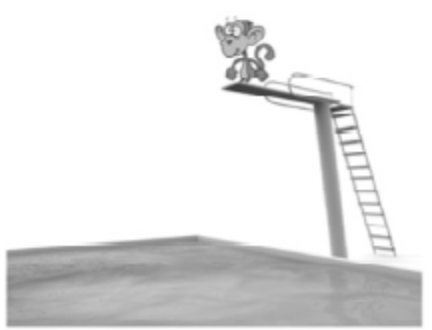
\includegraphics[width=4cm]{physics/figures/figure-unit-7-monkey.png}
\end{center}

If the monkey-earth system has \SI{3000}{J} of GPE when the monkey is at the top of the board, then how much kinetic energy would the monkey have at the bottom, right before he lands in the water? Assume air resistance is negligible.

\begin{randomizechoices}[norandomize]
    \correctchoice \SI{3000}{J} of KE
    \choice \SI{-3000}{J} of KE
    \choice \SI{0}{J} of KE
    \choice \SI{1500}{J} of KE
\end{randomizechoices}

\question
A \SI{2}{kg} brick falls to the ground from a \SI{3}{m} high roof. What is the work done of the brick by the force of gravity?

\begin{randomizechoices}[norandomize]
    \choice \SI{0}{J}
    \choice \SI{6}{J}
    \correctchoice \SI{60}{J}
    \choice \SI{600}{J}
\end{randomizechoices}

\question 
For an object sliding on a surface with friction, what effect will the frictional force have on this system?

\begin{randomizechoices}[norandomize]
    \correctchoice It will do work to remove energy from the system.
    \choice It will not affect the energy of the system.
    \choice It will do work to add energy to the system.
    \choice Not enough information is given to know the effects of friction on the system.
\end{randomizechoices}

\question
A \SI{6}{kg} book is resting on a shelf that is \SI{2}{m} above the floor. How much gravitational potential energy does the book-earth system have?

\begin{randomizechoices}[norandomize]
    \choice \SI{3}{J}
    \choice \SI{12}{J}
    \choice \SI{30}{J}
    \correctchoice \SI{120}{J}
\end{randomizechoices}

\question
The graphs below show the initial and final energies of a rock-earth system as the rock falls towards the earth. Which of the following statements could be inferred from the data in the graphs below?

\begin{center}
    \begin{tikzpicture}
    \begin{axis}[width=5cm,height=5cm,ymin=0,ymax=12,title=\textbf{Initial},
        symbolic x coords={$E_g$,$E_k$,$E_\mathrm{T}$},
        xtick=data,
        yticklabel=\empty]
        \addplot[ybar,fill=lightgray] coordinates {
            ($E_g$,8)
            ($E_k$,4)
            ($E_\mathrm{T}$,12)
        };
    \end{axis}
    \end{tikzpicture}%
    \hspace{1cm}
    \begin{tikzpicture}
    \begin{axis}[width=5cm,height=5cm,ymin=0,ymax=12,title=\textbf{Final},
        symbolic x coords={$E_g$,$E_k$,$E_\mathrm{T}$},
        xtick=data,
        yticklabel=\empty]
        \addplot[ybar,fill=lightgray] coordinates {
            ($E_g$,6)
            ($E_k$,4)
            ($E_\mathrm{T}$,8)
        };
    \end{axis}
    \end{tikzpicture}%
\end{center}

\begin{randomizechoices}[norandomize]
    \choice The decrease in kinetic energy is due to the external work of air resistance.
    \choice The decrease in potential energy is due to the external work of air resistance.
    \correctchoice The decrease in total energy is due to the external work of air resistance.
    \choice Since the kinetic energy was constant, there was no external work done on the system.
\end{randomizechoices}


\question
A father (\SI{100}{kg}) and his son (\SI{50}{kg}) are jogging at the same speed. Which statement is true about the kinetic energies (KE) of the father and the son? The father's KE is\dots

\begin{randomizechoices}[norandomize]
    \correctchoice Two times larger than the son's KE.
    \choice Four times larger than the son's KE.   
    \choice Two times smaller than the son's KE.
    \choice Four times smaller than the son's KE.
\end{randomizechoices}

\question
A \SI{60}{kg} bicyclist is initially at rest. How much energy does the bicycle have after the cyclist does \SI{120}{J} of work on the bicycle through pedaling? (Consider friction negligible).

\begin{randomizechoices}[norandomize]
    \choice \SI{2}{J}
    \choice \SI{4}{J}
    \choice \SI{60}{J}
    \correctchoice \SI{120}{J}
\end{randomizechoices}

\question
The diagram below depicts a 2-kg mass colliding with and sticking to a second box. What is the mass of the second box?

\begin{center}
    \begin{tikzpicture}
        \draw (0,0) -- (6,0) node[below,pos=0.5] {Before collision};
        \draw[thick] (1,0) rectangle ++(1.5,1) node[pos=0.5] {\SI{2}{kg}};
        \draw[thick,->] (2.5,0.5) -- ++(1.5,0) node[above,pos=0.7] {\SI{3}{m/s}};
        \draw[fill=gray] (4.5,0) rectangle ++(1,1);

        \begin{scope}[xshift=7cm]
            \draw (0,0) -- (6,0) node[below,pos=0.5] {After collision};
            \draw[thick] (1,0) rectangle ++(1.5,1) node[pos=0.5] {\SI{2}{kg}};
            \draw[fill=gray] (2.5,0) rectangle ++(1,1);
            \draw[thick,->] (3.5,0.5) -- ++(0.5,0) node[right] {\SI{1}{m/s}};
        \end{scope}
    \end{tikzpicture}
\end{center}

\begin{randomizechoices}[norandomize]
    \choice \SI{1}{kg}
    \choice \SI{2}{kg}
    \choice \SI{3}{kg}
    \correctchoice \SI{4}{kg}
\end{randomizechoices}

\clearpage

\begin{EnvUplevel}
In the diagram shown, a \SI{10}{kg} ball is fired with a velocity of \SI{500}{m/s} from a \SI{1000}{kg} cannon. 
\end{EnvUplevel}

\begin{center}
    \begin{tikzpicture}
        \draw[fill=lightgray] (0,-0.5) rectangle ++(2,1) node[pos=0.5] {cannon} node[below=0.5cm,pos=0.5] {$m = \SI{1000}{kg}$};
        \draw[thick,->] (0,0) -- ++(-0.5,0);
        \draw[fill] (4,0) circle (4pt) node[below=4pt] {$m = \SI{10}{kg}$};
        \draw[thick,->] (4,0) -- ++(2,0);
    \end{tikzpicture}
\end{center}

\question
What is the momentum of the system before the ball is fired and after the ball is fired?

\begin{randomizechoices}[norandomize]
    \correctchoice \SI{0}{kg\,m/s};\ \  \SI{0}{kg\,m/s}
    \choice \SI{1500}{kg\,m/s};\ \  \SI{500}{kg\,m/s}
    \choice \SI{0}{kg\,m/s};\ \  \SI{5000}{kg\,m/s}
    \choice \SI{5000}{kg\,m/s};\ \  \SI{5000}{kg\,m/s}
\end{randomizechoices}

\question 
What is the momentum of the cannon and of the ball after the ball is fired?

\begin{randomizechoices}[norandomize]
    \choice \SI{0}{kg\,m/s};\ \  \SI{0}{kg\,m/s}
    \choice \SI{0}{kg\,m/s};\ \  \SI{5000}{kg\,m/s}
    \correctchoice \SI{-5000}{kg\,m/s};\ \  \SI{5000}{kg\,m/s}
    \choice \SI{05000}{kg\,m/s};\ \  \SI{0}{kg\,m/s}
\end{randomizechoices}


\question
In the diagram below, scaled vectors represent the momentum of each of two masses, A and B, sliding toward each other on a frictionless, horizontal surface. Which scaled vector best represents the momentum of the system after the masses collide?

\begin{center}
    \begin{tikzpicture}
        \draw (0,0) -- (12,0) node[below,pos=0.5] {Frictionless surface};
        \draw[fill=gray] (1,0) rectangle ++(1,1) node[pos=0.5,below=0.5cm] {Mass A} (10,0) rectangle ++(1,1) node[pos=0.5,below=0.5cm] {Mass B};
        \draw[->,thick] (2,0.5) -- ++(4,0); 
        \draw[->,thick] (10,0.5) -- ++(-1,0);
    \end{tikzpicture}
\end{center}

\begin{randomizeoneparchoices}[norandomize]
    \choice \tikz{\draw[->,thick] (0,0) -- (-1,0);}
    \correctchoice \tikz{\draw[->,thick] (0,0) -- (+3,0);}
    \choice \tikz{\draw[->,thick] (0,0) -- (-4,0);}
    \choice \tikz{\draw[->,thick] (0,0) -- (+4,0);}
\end{randomizeoneparchoices}

\bigskip

\hrule
\hrule



\clearpage
\printkeytable

\end{questions}
\end{document}


\bigskip

\begin{EnvUplevel}
    \centering
    \textbf{PART II. Continued Science Mastery (CSM) Questions}
\end{EnvUplevel}

\question \label{N3JMlC}
In athletics, a ``hammer'' is not construction tool but a 4-kilogram metal ball connected to a handle by a steel wire. Suppose Anita spins the hammer in a circular path, supplying a centripetal force of \SI{320}{N} and giving the hammer a tangential speed of \SI{12}{m/s}. Besides centripetal acceleration and the mass of the hammer, what other information is needed to calculate the centripetal force?


\begin{minipage}{0.4\textwidth}
    \centering
	\begin{randomizechoices}[norandomize]
		\correctchoice radius of curvature
		\choice tangential speed
		\choice Anita's mass
		\choice acceleration due to gravity
	\end{randomizechoices}
\end{minipage}%
\hspace{1cm}
\begin{minipage}{0.6\textwidth}
    \centering
\begin{center}
    \begin{tikzpicture}
        \begin{axis}[
            width=8cm,height=6cm,
            axis line style={draw=none},
            axis equal image,
            ticks=none,
            axis lines=middle,
            xmin=-1.1,xmax=1.6,
            ymin=-0.2,ymax=1.1,
            clip=true,
        ]
        % \clip (-1.1,-0.2) rectangle ++(2.2,1.4);
        \draw[gray,dashed] (0,0) circle (1);
        \begin{scope}[shift={(axis direction cs: 0,-0.05)}]
            \draw[gray,<->] (0,0) -- ({cos(0)},{sin(0)}) node[pos=0.5,below] {$r$};
        \end{scope}
        \draw[Green,very thick,->] ({cos(0)},{sin(0)}) -- ++(axis direction cs: -0.4,0) node[black,above=3pt] {$a_{\text{c}}$};
        \draw[red,very thick,->] ({cos(0)},{sin(0)}) -- ++(axis direction cs: 0,0.7) node[black,pos=1.1] {$\SI{12}{m/s}$};
        \fill (0,0) circle (1pt);
        \fill ({cos(0)},{sin(0)}) circle (3pt) node[right] {$\SI{4.0}{kg}$};
    \end{axis}
    \end{tikzpicture}
    \end{center}
\end{minipage}

\question
A fly tethered by a spider web is undergoing uniform circular motion. At the instant the fly's velocity vector points to the right, what is the direction of the centripetal acceleration?

\begin{minipage}{6cm}
    \centering
    \begin{randomizechoices}[norandomize]
        \correctchoice up
        \choice down
        \choice left
        \choice right
    \end{randomizechoices}
\end{minipage}%
\begin{minipage}{6cm}
    \centering
	\begin{tikzpicture}
		\draw[dashed] (0,0) circle (2);
		\draw[<->] (0,-0.5) node[below] {down} -- ++(0,1) node[above] {up};
		\draw[<->] (-0.5,0) node[left] {left} -- ++(1,0) node[right] {right};
		\draw[->,ultra thick] (0,-2) -- ++(1.5,0) node[right] {$\bvec{v}$};
		\fill (0,-2) circle (3pt);
	\end{tikzpicture}
\end{minipage}

\clearpage
\question
A tennis ball is launched straight up into the air from the reference point of the ground. At the ball's maximum height, velocity is \fillin[zero].

\begin{randomizechoices}[norandomize]
    \correctchoice zero
    \choice maximum
    \choice increasing
    \choice decreasing
\end{randomizechoices}

\question
After a projectile is launched in the air, in which direction does it experience constant, non-zero acceleration? Ignore air resistance.

\begin{randomizechoices}[norandomize]
	\correctchoice The $y$ direction
	\choice The $x$ direction
	\choice Neither direction
	\choice Both the $x$ and $y$ direction
\end{randomizechoices}

\question
An object on a string is moving around a circle in a counter-clockwise direction as shown below:

\begin{center}
	\begin{tikzpicture}[scale=0.9]
		\draw (0,0) circle (1);
		\fill ({-cos(45)},{sin(45)}) circle (3pt) node[above left=-2pt] {P};
		\draw[->,ultra thick] (4,{cos(45)}) -- ++({-2*cos(45)},{-2*sin(45)}) node[pos=1.1] {\large A};
		\draw[->,ultra thick] (3.5,-{cos(45)}) node[below left=-1mm] {\large B} -- ++({2*cos(45)},{2*sin(45)});
		\draw[->,ultra thick] (5.5,{cos(45)}) -- ++({2*cos(45)},{-2*sin(45)}) node[pos=1.1] {\large C};
		\draw[<-,ultra thick] (6.5,{cos(45)}) -- ++({2*cos(45)},{-2*sin(45)}) node[pos=1.15] {\large D};
		\draw[->,ultra thick] (9,{cos(45)}) -- ++(0,{-2*sin(45)}) node[pos=1.15] {\large E};
	\end{tikzpicture}
\end{center}

If the string breaks when the object is at point P, the object will fly off in the direction of which arrow?

\begin{randomizeoneparchoices}[norandomize]
	\correctchoice Arrow A
	\choice Arrow B
	\choice Arrow C
	\choice Arrow D
	\choice Arrow E
\end{randomizeoneparchoices}